\subsection{Autoencoder for feature extraction}
An Autoencoder is a neural network of multilayer structure that can learn
efficient coding of similar data, that allows reconstructing with an acceptable
accuracy. It consists of two parts, an encoder and a decoder, which are
symmetrical to each other, i.e., the decoder is built up from the same layers as
the encoder but in reverse order (see Fig. \ref{ae}). The two overlap in the
middle of the network forming a ``mirror''. The middle layer will later contain
the encoded data, which lie in the so called \textit{latent space}. This layer
has the function of a ``bottleneck'', it is significantly smaller than the input
and output layer of the autoencoder. Learning is performed layer after layer and
has the goal is to create an output as close to the corresponding input as
possible, hence the name \textit{auto}encoder. The bottleneck in the middle
forces the encoder to abstract these vectors and map them to a smaller
representation. The decoder then tries to reconstruct the original data. For
feature extraction purposes, one is merely interested in the encoder part which
will be fed into the classification system.

Autoencoders are very well suited for extracting features from faces, because an
image of a face can be described much more space-savingly if you do not save the
RGB values of all pixels, but only the features that distinguish a certain face
from another. So, if the network's structure and the size of the bottleneck are
cleverly chosen, the autoencoder should automatically learn to map the features
of the faces in latent space. 

\begin{figure}[h]
  \centering
  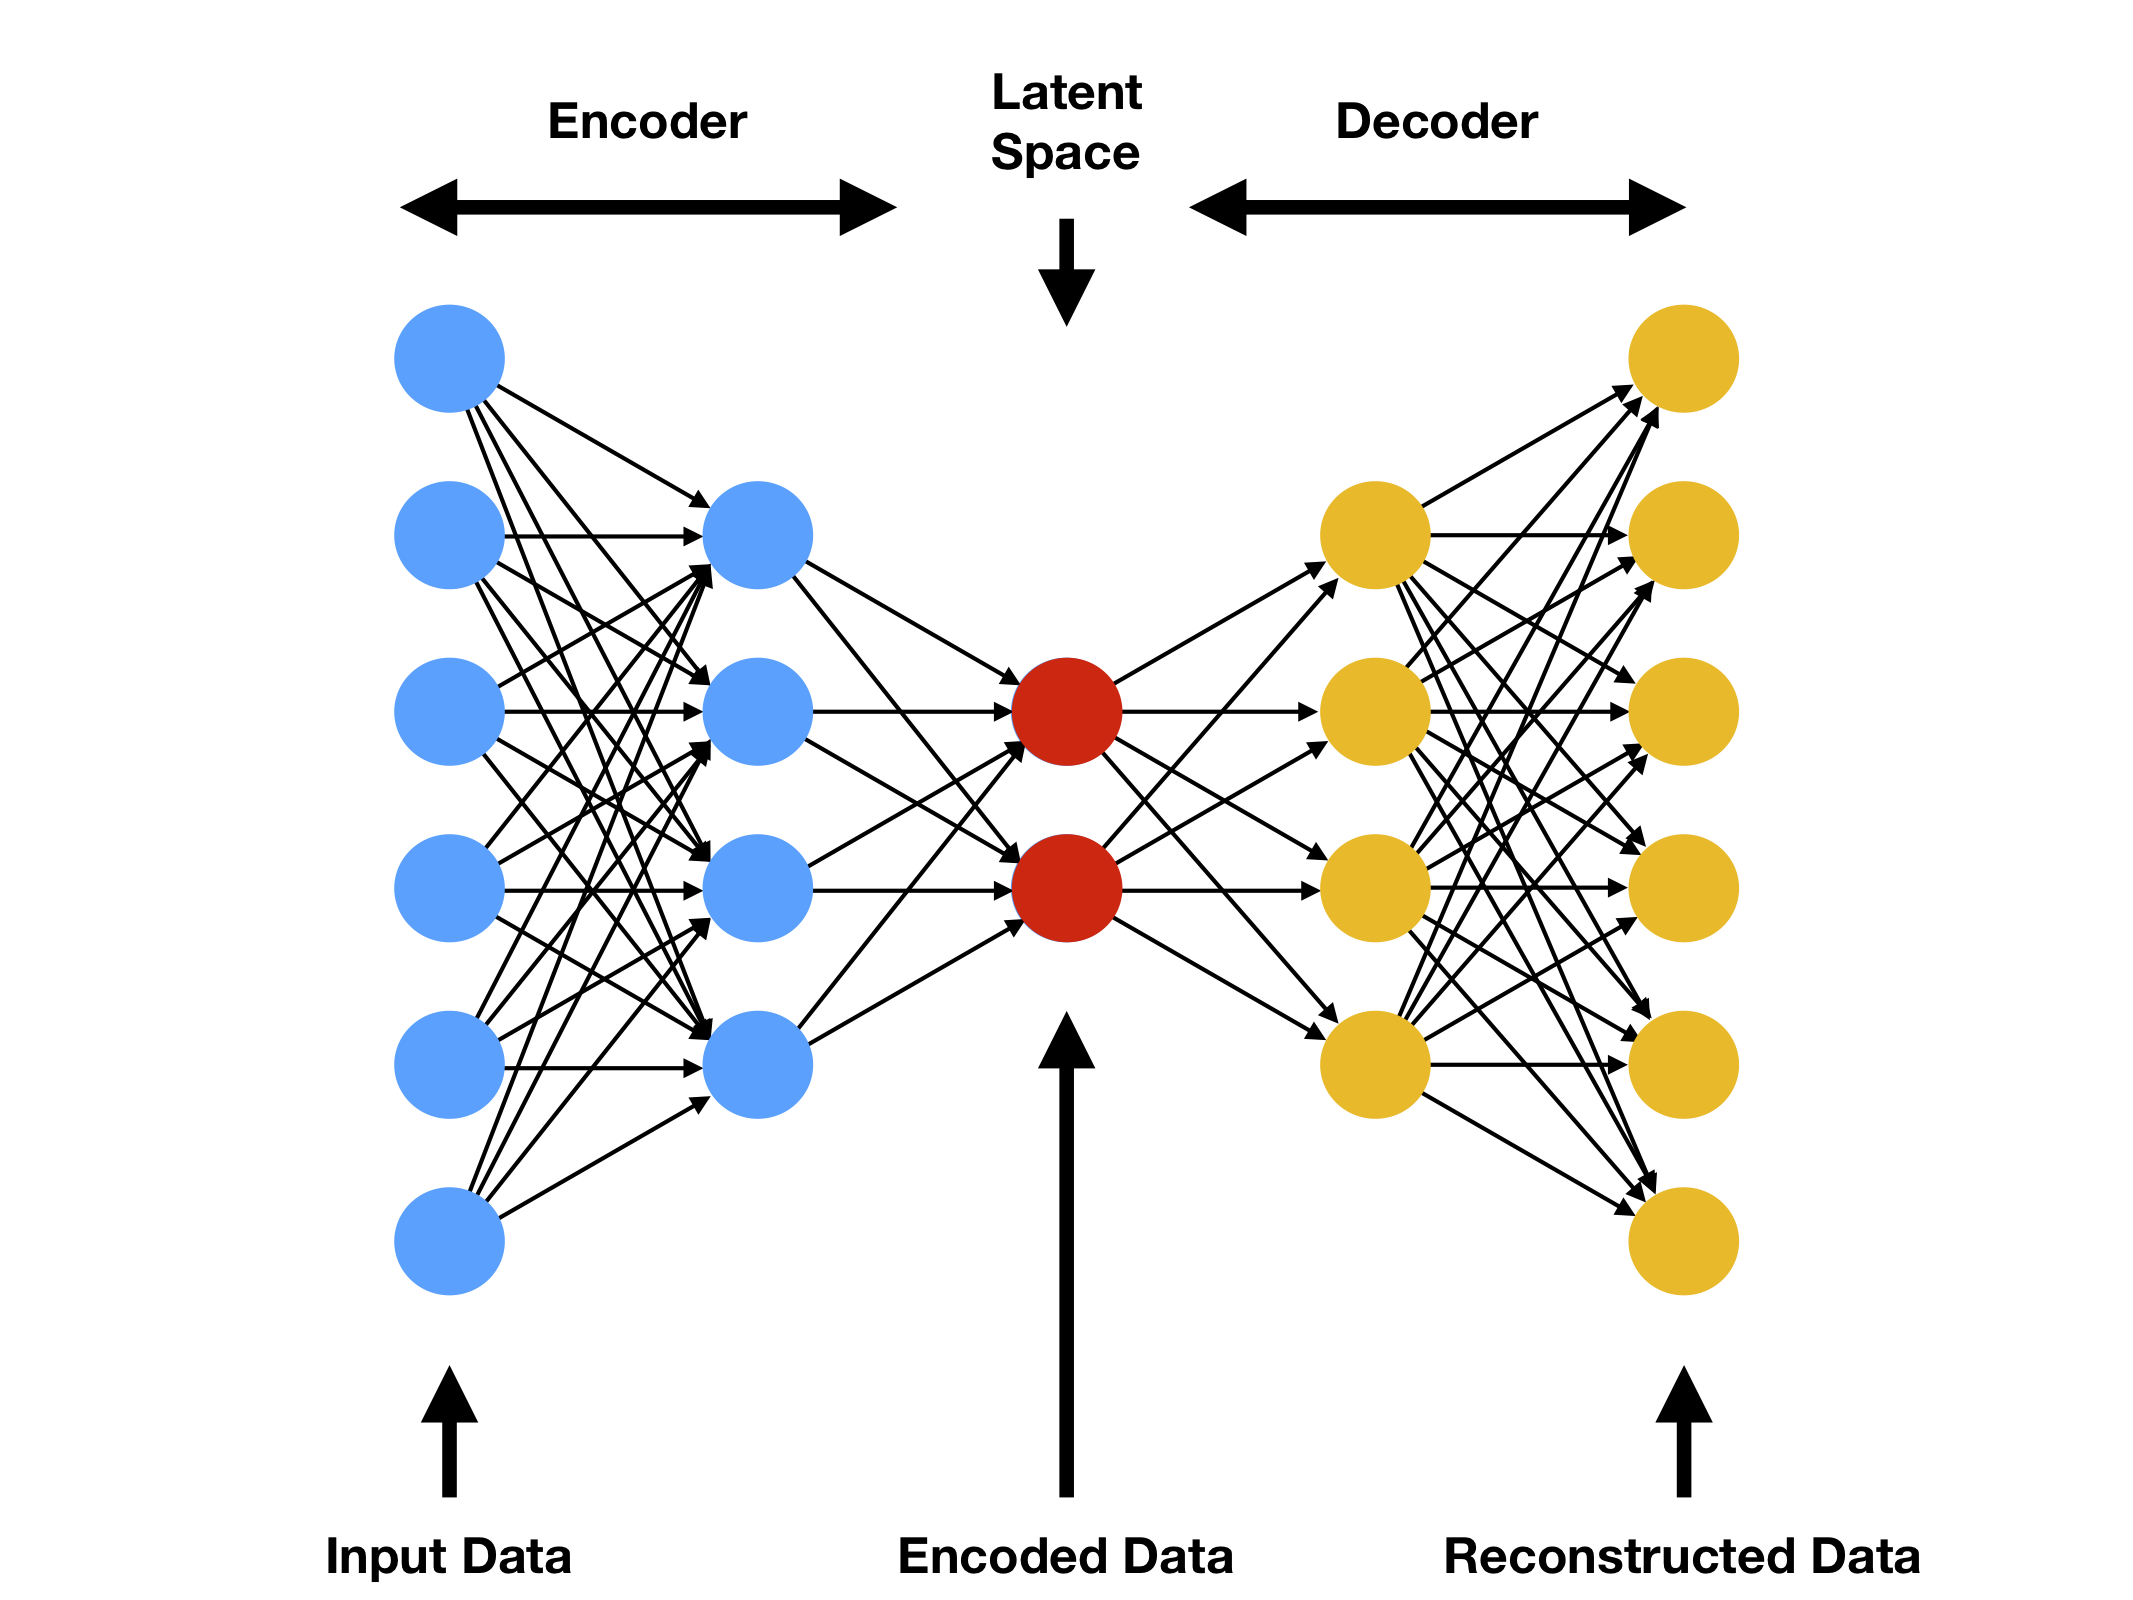
\includegraphics[width=\columnwidth]{ae.png}
  \caption{Structure of an autoencoder}
  \label{ae}
\end{figure}

\subsection{Convolutional Neural Network}
As images are encoded in this project, I will be using an Autoencoder based on
Convolutional Neural Networks (CNN). This type of network is well suited for the
analysis of images, because in the first layers of the network small sections of
the present image are processed independently. Only in later layers are these
sections then merged together, so that the network can detect larger and more
complex structures of the image with each convolution layer without having to
look at the image in its entirety from the beginning. This saves a lot of
resources and achieves very good results in general. 

A CNN generally consists of three types of layers: \textit{Convolutions},
subsampling or \textit{pooling layers}, and conventional \textit{fully-connected
layers}.

Convolutions maintain the width and height of the three-dimensional neuron
matrix they receive, and only change the depth. They have a filter kernel that
applies any number of filters to any point of the obtained matrix. The result
for each filter is written to the output matrix at the same point, so that the
depth of the output matrix corresponds to the number of filters, but the width
and height remain unchanged. Learning is performed by finding optimal
convolution filter parameters.

Pooling layers reduce the width and height of the obtained matrix. They do this
by pooling adjacent points of the matrix. In \textit{Max-Pooling} for instance,
only the largest value for each 2×2 square is written to the output matrix.
Thus, the height and width of the matrix are halved, but the depth remains
unchanged. This has the purpose of discarding superfluous data so that later
convolutions can recognize larger structures.

A CNN consists of a sequence of one or more convolutions, followed by a pooling
layer. If the size of the neuron matrix is sufficiently reduced, one or more
fully-connected layers follow in order to finally evaluate the data and
categorize it. Each layer is usually followed by the ReLU activation function. 
